% !TEX encoding = UTF-8
% !TEX TS-program = pdflatex
% !TEX root = ../tesi.tex

%**************************************************************
\chapter{Contesto aziendale}
\label{cap:introduzione}
%**************************************************************

%**************************************************************
\section{Lab Network}

\begin{figure}[h]
	\begin{center}
	
\includegraphics[scale=0.4]{immagini/LOGO_LABNETWORK.png}
	\caption{Logo \lab{}}
	\end{center}
\end{figure}

\lab{} nasce nel 2016 con lo scopo di aiutare le imprese ad innovare prodotti e processi attraverso la competenza concreta dei laboratori, sfruttando le potenzialità dei moderni strumenti digitali.

\section{Organizzazione aziendale}
Descrizione dei processi aziendali, dell'organigramma e della metodologia di lavoro che l'azienda ha adottato e affinato negli anni.
Tecnologie utilizzate

\newpage
\section{Prodotti e servizi}
\subsection{Prodotti}
\textbf{VITRUVIAN GAME – Wingsuit VR}\\
\begin{figure}[h]
\begin{center}
	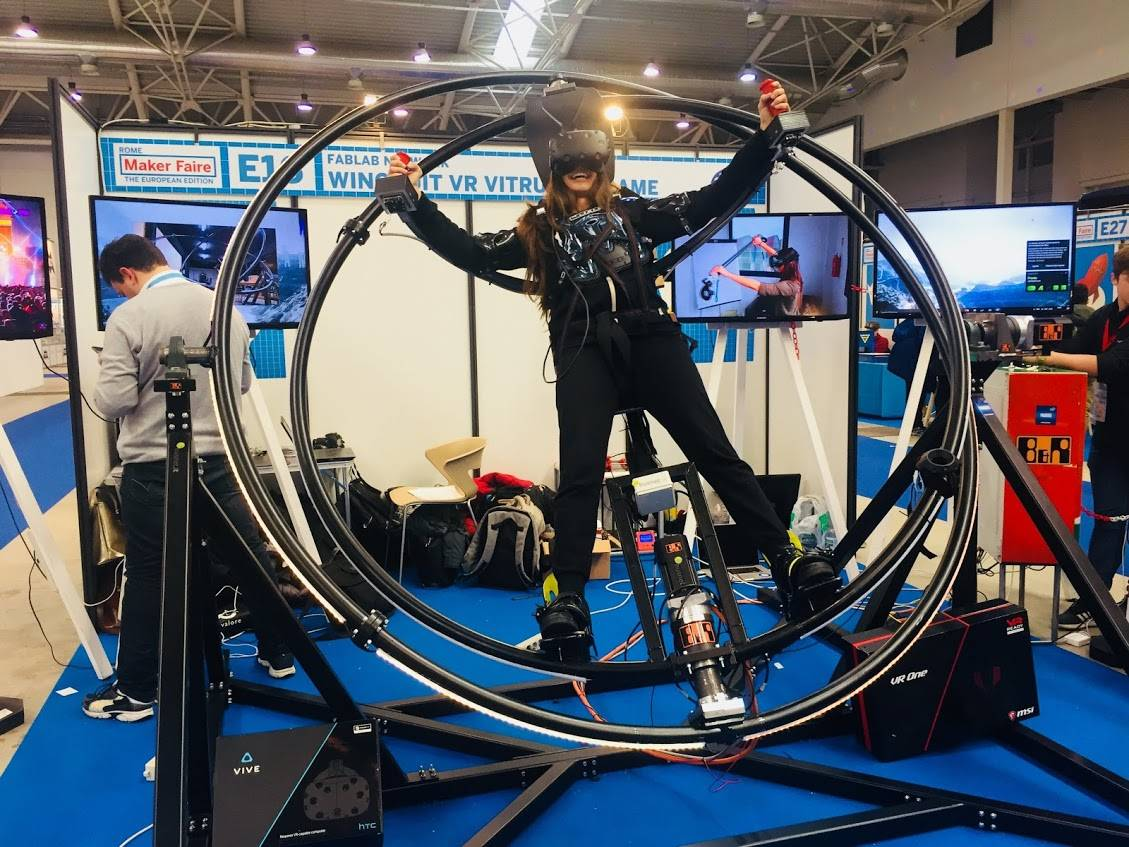
\includegraphics[scale=0.2]{immagini/vitruvian.jpg}
	\caption{Vitruvian Game}
\end{center}
\end{figure}
\\
Dalla collaborazione con Intel\textsuperscript{\textregistered} nasce il simulatore di volo con tuta alare ispirato al capolavoro di Leonardo.\\
Il progetto prevede l'utilizzo del visore HTC Vive affiancato ad uno scenario virtuale sviluppato su piattaforma \textit{Unity}. Per i movimenti sugli assi sono stati impiegati dei motori per automazione industriale.
\\
\\
\textbf{FabKey}
\\
La serratura smart connessa ad internet. Permette l'apertura di una porta controllando una lista di accessi presente in cloud. Funziona tramite tag \gls{NFC} o barcode. Il prodotto è rivolto principalmente ai \gls{FabLab}, ma si adatta facilmente a qualsiasi contesto in cui sia richiesto il controllo degli accessi.
\\
\\
\textbf{Smart Meter}
\\
Un metro 4.0 capace di misurare superfici complesse e inviare direttamente i dati al software gestionale, in aggiunta anche il monitoraggio in tempo reale di quando, dove e per quanto tempo è stato utilizzato dal singolo addetto.


\subsection{Servizi}
I servizi che \lab{} offre ai propri clienti sono:
\begin{itemize}
\item \textbf{Progettazione:} corsi di formazione su misura, \gls{counseling} e \gls{workshop} per imparare a sfruttare in modo professionale: 3D Printing, schede elettroniche, \gls{cz}, realtà virtuale e aumentata, sviluppo App, prototipazione, \gls{bigd}, \gls{iot} ecc.
\item \textbf{Noleggio:} Kit e attrezzature come stampanti 3D, schede elettroniche (\gls{arduino}, \gls{rpi}, Intel) visori VR, pc e notebook, videoproiettori; affitto aule didattiche per \gls{makers} e industria 4.0.
\item \textbf{Personale qualificato:} per i clienti sono a disposizione docenti, tecnici di laboratorio e consulenti specializzati nei principali ambiti di innovazione digitale.
\item \textbf{Assistenza:} pianificazione e costruzione su misura di progetti innovativi sviluppando idee imprenditoriali.
\end{itemize}

\section{Lab Network e innovazione}
In questa sezione descriverò il rapporto che \lab{} ha con l'innovazione, ovvero come investe su di essa in termini di prodotti, servizi e personale.